% !TEX root = ejb-web.tex
%!TEX encoding = UTF-8 Unicode
\ifx\setbeamertemplate\undefined
\documentclass[handout]{beamer}
\fi
\usepackage{amsmath}

\usepackage{mathtools}
\mathtoolsset{showonlyrefs}
\usepackage{mathrsfs}

\usepackage[multidot]{grffile}

\usepackage{xspace}
\usepackage{upgreek}
\newcommand\xsb{$\upchi$SB\xspace}
\newlength{\imagecolumnwidth}

\usepackage[absolute,overlay]{textpos}

\usepackage{slashed}
\newcommand\dslash{\slashed{\partial}}

\usepackage{bbold}
\newcommand\one{\mathbb{1}}

\usepackage{multirow}

\newcommand\bs\boldsymbol

\newcommand \Sx[1] {S_{\textnormal{#1}}}
\newcommand \Sg[2] {\mathrm{#1}(#2)}
\newcommand \SU[1] {\Sg{SU}{#1}}
\newcommand \SO[1] {\Sg{SO}{#1}}
\newcommand \Sp[1] {\Sg{Sp}{#1}}
\newcommand \Uone {\Sg{U}{1}}

\newcommand\pb{\overline{\psi}}
\newcommand \bigL {\mathscr{L}}
\newcommand \lag[1] {\bigL_{\mathrm{#1}}}

\newcommand\sptn{Sp($2N$)\xspace}
\newcommand\dee{\mathrm{d}}
\newcommand\eee{\mathcal{E}}
\newcommand\www{\mathcal{W}}
\DeclareMathOperator\tr{tr}
\DeclareMathOperator\real{Re}
\newcommand\Nf{N_{\mathrm{f}}}

%\usepackage{beamerthemesplit} %Activate for custom appearance
\setbeamertemplate{navigation symbols}{}%remove navigation symbols

\usefonttheme[onlymath]{serif}
\usepackage{fontspec,xltxtra,xunicode}
\defaultfontfeatures{Mapping=tex-text}
\setsansfont[Scale=MatchLowercase,Mapping=tex-text]{Futura}
\setbeamerfont{structure}{family=\fontspec{Cosmos BQ}}
\definecolor{swanseablue}{RGB}{36,47,96}
\setbeamercolor{structure}{fg=swanseablue}
 \setbeamertemplate{itemize item}{•}
 \setbeamertemplate{itemize subitem}{--}
 \setbeamercolor{itemize item}{fg=black}
 \setbeamercolor{itemize subitem}{fg=black}


\newfontfamily{\J}[Scale=0.85]{Osaka}

\newcommand\disappear[1]{}
\title{Performance optimisation of research codes for the Supercomputing Wales programme: three case studies
}
\author{{\large Ed Bennett}
	\\{\small@QuantumofEd}
	\\\vspace{16pt}
	\hfill
	\parbox{0.22\textwidth}{\centering
\includegraphics[height=36pt]{swansea}\\\small @SwanseaUni}
	\parbox{0.44\textwidth}{\centering
\includegraphics[height=24pt]{scw}\\\small @SuperCompWales}
	\parbox{0.22\textwidth}{\centering
\includegraphics[height=36pt]{sa2c}\\\small @sa2c\_swansea} }
\date{HPC-LEAP Conference, Cambridge University\\11 July 2018}

\newcommand\Wider[2][3em]{%
\makebox[\linewidth][c]{%
  \begin{minipage}{\dimexpr\paperwidth-#1\relax}
  \raggedright#2
  \end{minipage}%
  }%
}



\newcommand\FrameText[1]{%
  \begin{textblock*}{0.9\paperwidth}(3pt, 0.99\textheight)
    \raggedright #1\hspace{.5em}
  \end{textblock*}}

\newcommand \sechead[1] {\frame{\vfill\Huge \centering\usebeamerfont{structure}\color{swanseablue}#1\vfill\null}}

\usebackgroundtemplate%
{%
	
\includegraphics[width=\paperwidth,height=\paperheight]{bg}%
}
\setbeamertemplate{footline}{
	\vspace{1.0cm}
}


  
\begin{document}

\frame{\titlepage}

\frame{
	\frametitle{In this talk}
	
	\begin{itemize}%[<+->]
		\item The Supercomputing Wales programme
		\item What is a Research Software Engineer?
		\item Case studies:
		\begin{itemize}
			\item Throughput optimization of a life sciences application
			\item Improving parallel efficiency of a CFD application
			\item Parallelising a lattice field theory code
		\end{itemize}
	\end{itemize}
}

\frame {
	\frametitle{The Supercomputing Wales programme}

	\begin{itemize}[<+->]
		\item £15m investment by EU, Welsh Government, and four Welsh Universities
		\begin{itemize}[<+->]
			\item Cardiff
			\item Swansea
			\item Aberystwyth
			\item Bangor
		\end{itemize}
		\item Two HPC facilities
		\begin{itemize}[<+->]
			\item 12,000 Skylake cores
			\item 34 Nvidia V100 GPUs
			\item 2 Bullion Analytics Factories
		\end{itemize}
		\item 15 Research Software Engineers
	\end{itemize}
}


\frame {
	\frametitle{What is a Research Software Engineer?}

	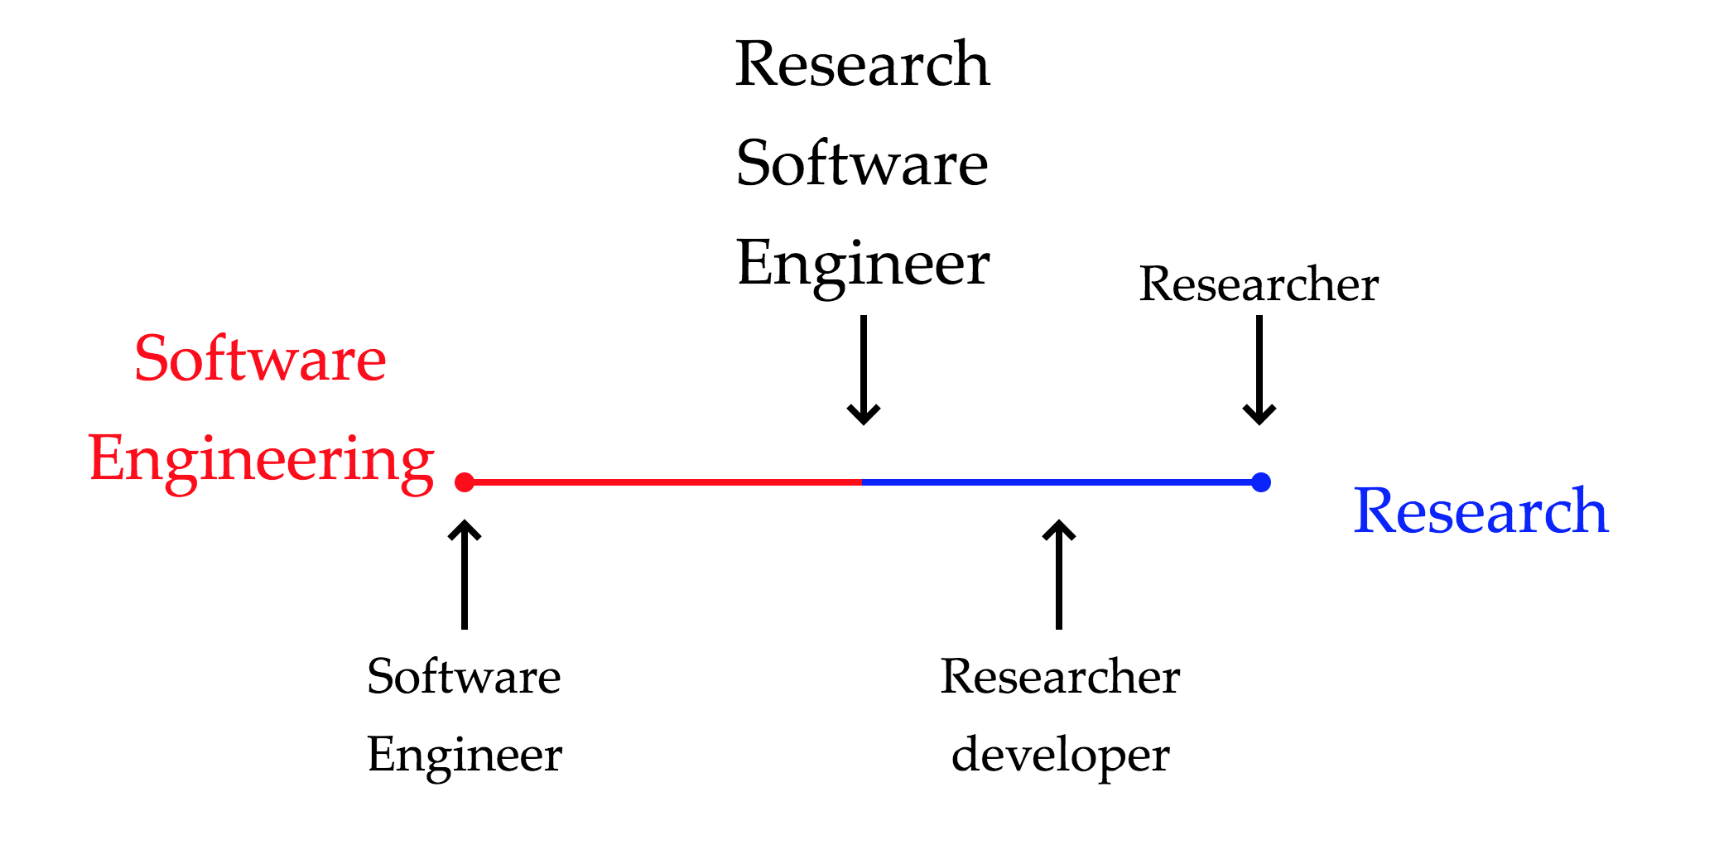
\includegraphics[width=\textwidth]{rse.png}
	\null\hfill(from Simon Hettrick, https://goo.gl/znRRzb)
}

\frame {
	\frametitle{Supercomputing Wales RSEs}

	\begin{itemize}[<+->]
		\item RSEs:
		\begin{itemize}[<+->]
			\item Know software engineering
			\item Know research
			\item Develop software for research
		\end{itemize}
		\item Supercomputing Wales RSEs:
		\begin{itemize}[<+->]
			\item Do all this
			\item Know about HPC
			\item Adapt, optimize, and benchmark research software for HPC
		\end{itemize}
	\end{itemize}
}


\frame {
	\frametitle{Throughput optimisation for life sciences}

	\centering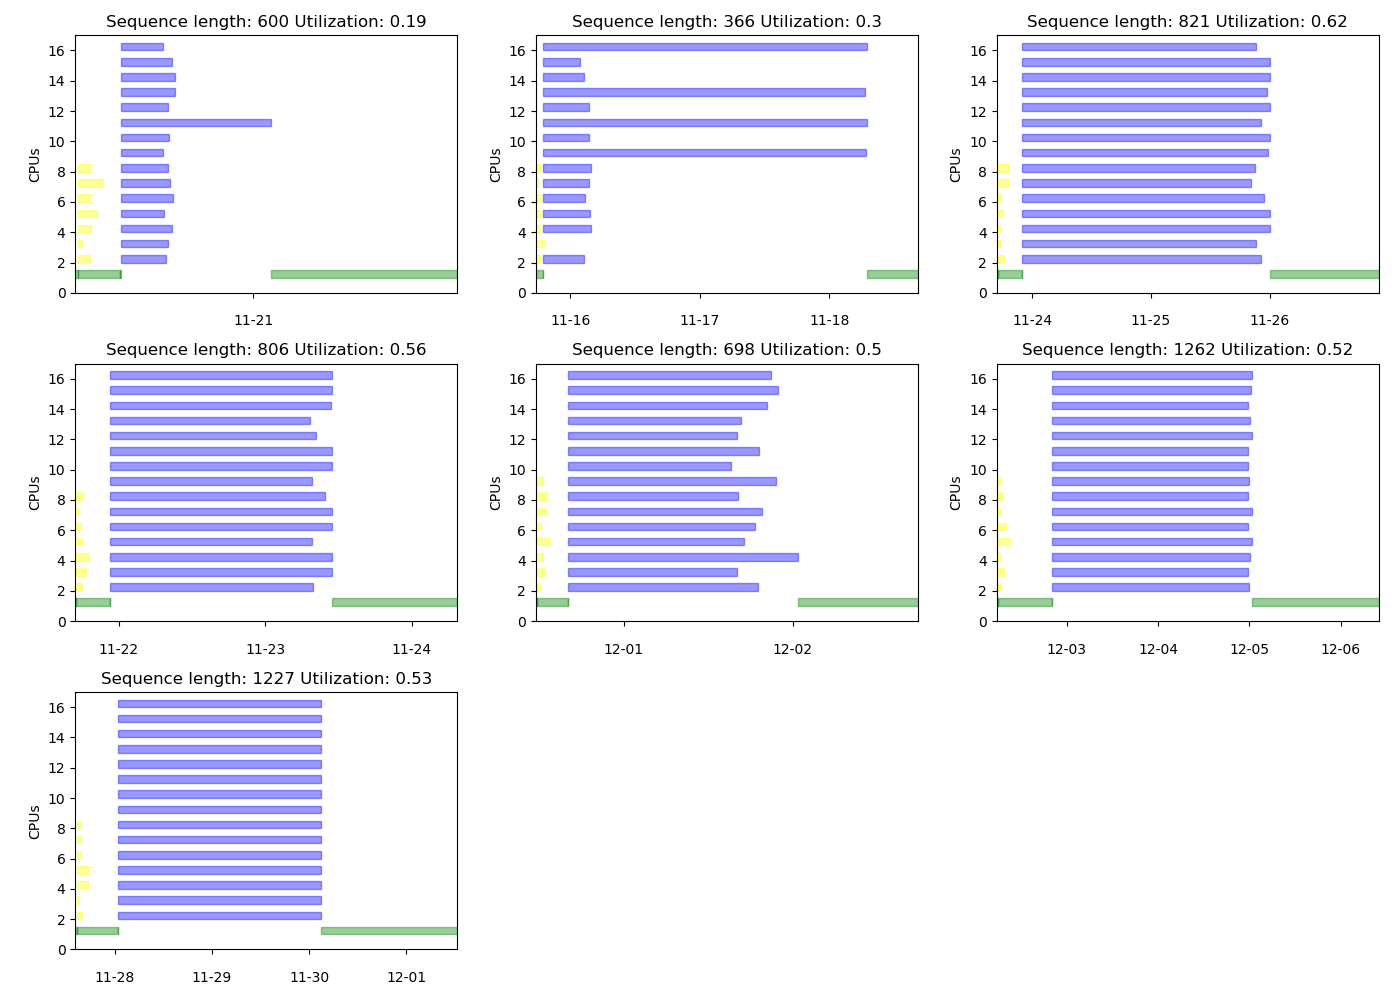
\includegraphics[width=0.9\textwidth]{ls_unopt}
}

\frame {
	\frametitle{Options considered}

	\begin{itemize}[<+->]
		\item Serialise
		\item Separate jobs, SLURM dependencies
		\item Allocate a single job, run many jobs within it
		\begin{itemize}[<+->]
			\item Require a queue manager to organise this
		\end{itemize}
	\end{itemize}
}

\frame {
	\frametitle{METAQ (https://git.io/fNUxC)}

	\begin{itemize}[<+->]
		\item Written in bash
		\item Filesystem-based
		\item No support for dependencies
		\begin{itemize}[<+->]
			\item Now implemented
		\end{itemize}
	\end{itemize}
}

\frame {
	\frametitle{Initial results of throughput optimisation}

	\Wider{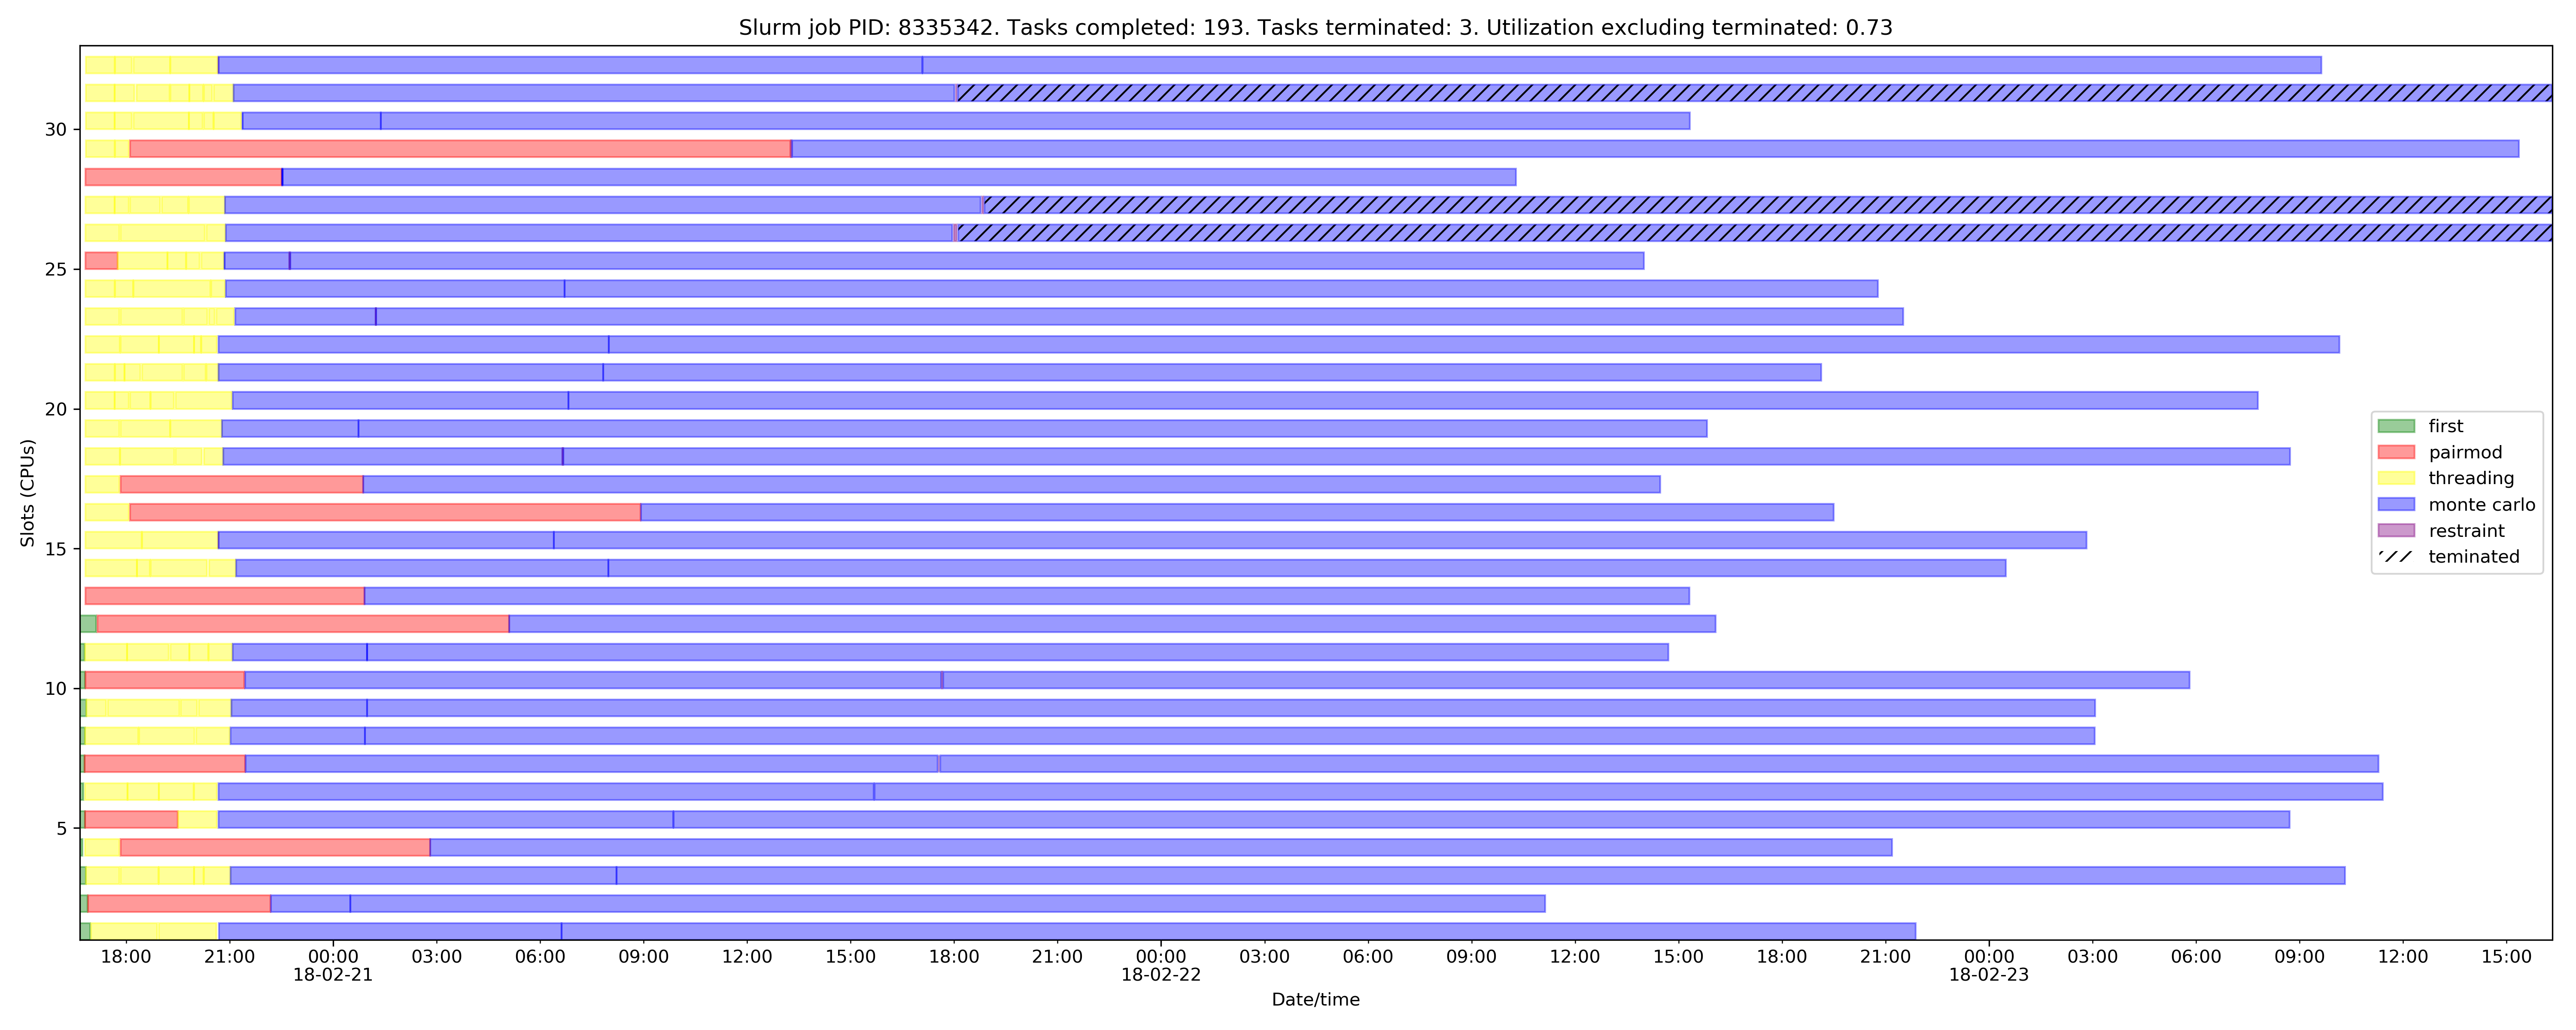
\includegraphics[width=\textwidth]{ls_opt}}
}

\frame {
	\frametitle{Ongoing work}

	\begin{itemize}[<+->]
		\item Predictions of runtime for each job step
		\item Collecting data from current runs to allow this
	\end{itemize}
}


\frame {
	\frametitle{Parallel optimisation of computational fluid dynamics software}

	\begin{itemize}[<+->]
		\item Solver for the 2D Boltzmann equation
		\begin{itemize}[<+->]
			\item BGK operator
			\item Two-step discontinuous Taylor--Galerkin
		\end{itemize}
		\item Position and velocity degrees of freedom
		\item Initially position-space parallelised (domain decomposition)
		\begin{itemize}
			\item Memory bound
			\item Performance not explicitly considered
		\end{itemize}
		\item Fortran 77 code
	\end{itemize}
}

\frame {
	\frametitle{Initial performance, 30k elements}

	\centering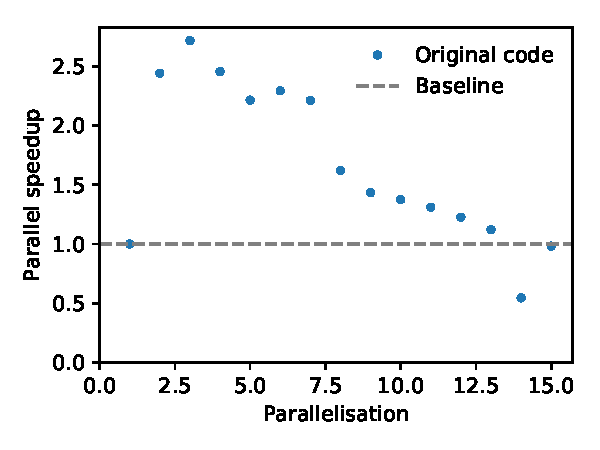
\includegraphics[width=0.95\textwidth]{cfd_unopt}
}

\frame {
	\frametitle{Optimisations implemented}
	
	\begin{itemize}[<+->]
		\item Parallelise in velocity space
		\begin{itemize}[<+->]
			\item Less communication on this axis
		\end{itemize}
		\item Optimise domain decomposition
		\begin{itemize}[<+->]
			\item Better load balancing
			\item Less communication
		\end{itemize}
		
	\end{itemize}
}

\frame {
	\frametitle{Optimised performance, 30k elements}

	\centering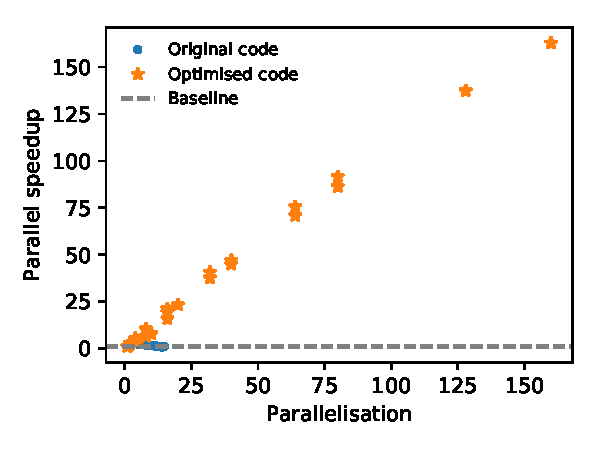
\includegraphics[width=0.95\textwidth]{cfd_opt1}
}

\frame {
	\frametitle{Optimised performance, 400k elements}
	
	\centering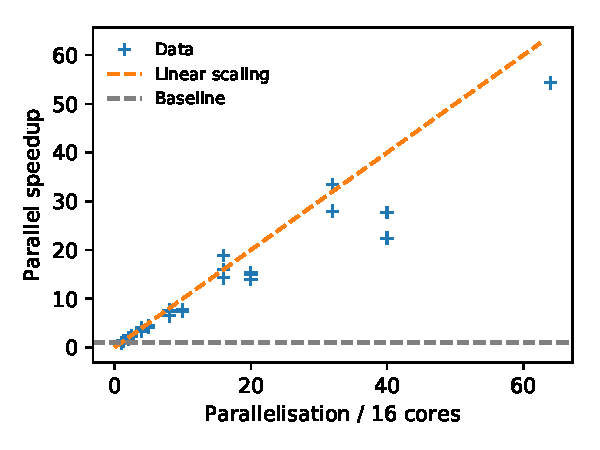
\includegraphics[width=0.95\textwidth]{cfd_opt2}
}


\frame {
	\frametitle{Parallelising lattice field theory code}

	\begin{itemize}[<+->]
		\item 2+1d Thirring model
		\item RHMC algorithm
		\item Serial Fortran 77 (and FORTRAN IV) code
		\item Domain Wall Fermions
		\begin{itemize}[<+->]
			\item Highly vectorisable
		\end{itemize}
		\item Need for:
		\begin{itemize}[<+->]
			\item Larger volumes $\Rightarrow$ longer time per iteration
			\item Stronger coupling $\Rightarrow$ more iterations
		\end{itemize}
		\item $\Rightarrow$ Need parallelism
	\end{itemize}
}

\begin{frame}[fragile]
	\frametitle{Initial tests}

	\begin{itemize}[<+->]
		\item Tune compiler options: 40\% performance improvement
		\begin{itemize}[<+->]
			\item Before: \verb|ifort -O3 -heap-arrays|
			\item After: \scriptsize\verb|ifort -ipo -no-prec-div -fp-model fast=2 -xHost -O3 -heap-arrays|
		\end{itemize}
		\item Automatic multithreading (\verb|-parallel|)
		\begin{itemize}[<+->]
			\item Near linear scaling to 4 threads
			\item Rapid fall off afterwards
		\end{itemize}
		\item Deliver $\sim5\times$ improvement to researcher before starting MPI
	\end{itemize}
\end{frame}

\begin{frame}[fragile]
	\frametitle{Refactoring}

	\begin{itemize}[<+->]
		\item Implement regression testing
		\item Add per-site random numbers
		\item Remove indirection
		\item Move to free-form Fortran
		\item Replace loop operations with array operations where possible
		\begin{verbatim}
      do 1000 i=1,10000
 1000   sum_x = sum_x + x(i)
\end{verbatim}
becomes
\begin{verbatim}
sum_x = sum(x)
\end{verbatim}

		\item \verb|implicit none|
		\item \verb|common| blocks $\rightarrow$ modules
		\item Global \verb|parameter|s $\rightarrow$ module
	\end{itemize}
\end{frame}

\frame {
	\frametitle{Adding MPI}

	\begin{itemize}[<+->]
		\item 1-site halo in space-time
		\item Explicit halo communications in serial
		\item Add parallel communications
		\begin{itemize}[<+->]
			\item Broadcast parameters
			\item Use MPI-IO
			\item Communicate halo 
			\item Use collective reductions (sum, max, etc.)
			\item Seed RNG based on rank
			\item Handle correlation functions
		\end{itemize}
		\item Test, test, test
	\end{itemize}
}

\frame {
	\frametitle{MPI Perforamnce}
	
	\centering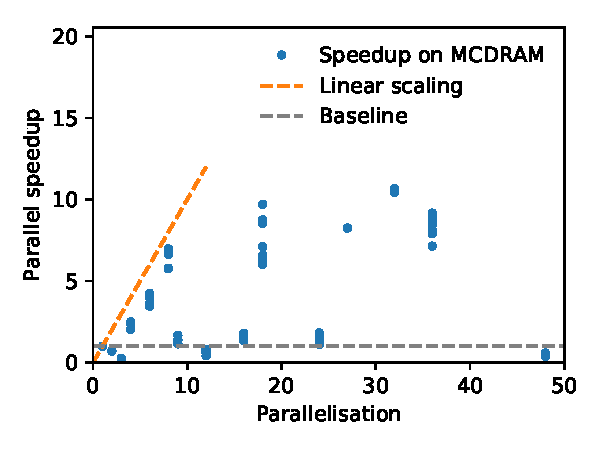
\includegraphics[width=0.95\textwidth]{lft_mpi}
}

\frame {
	\frametitle{Ongoing work}
	
	\begin{itemize}[<+->]
		\item Full physics tests
		\item Investigate unexpected MPI slowdowns
		\item Test combining with automated multithreading
	\end{itemize}
}

\frame {
	\frametitle{Other projects}
	
	\begin{itemize}[<+->]
		\item Port openQCD to AVX 512 (KNL, Skylake)
		\item Port Windows GPU code to Linux
		\item Prepare benchmark report supporting PRACE application
		\item Develop accessible desktop client for HPC
		\item Group theory-based memory compression for Sp($2N$) lattice gauge theory
		\item Speeding up inter-process communication between Python and C++
	\end{itemize}

}

\frame {
	\frametitle{Thanks for listening!}
	
	\begin{itemize}
		\item<2-> Interested?
		\item<3-> Currently recruiting
		\item<4-> bit.ly/swansea-rse-2018
		\item<5-> Deadline: 20 July (next Friday)
	\end{itemize}

	\Wider[0em]{\includegraphics[width=\textwidth]{swansea-panorama}}
}

\end{document}
